\Chapter{Database Design}

The CELORS implements an object/relational mapping (ORM) framework through Hibernate. Hibernate provides the bridge between the database, which is MySQL, and the Java application by storing application objects in the database, rather than writing and maintaining an abundance of code to store and retrieve objects. In short, object/relational mapping (ORM) is the automated persistence of objects to the tables in a relational database. Hibernate uses required metadata to describe the mapping between the objects and the database. Table~\ref{table:staff_metadata} is a mapping metadata for the staff table.

\vspace{3em}

\begin{table}[H]
\caption{Staff Table Metadata}\label{table:staff_metadata}
	\textbf{ }
\small
\begin{tabular}{p{13cm}}
\begin{verbatim}
<?xml version='1.0'?>
<!DOCTYPE hibernate-mapping PUBLIC 
         "-//Hibernate/Hibernate Mapping DTD 3.0//EN" 
         "http://hibernate.sourceforge.net/hibernate-mapping-3.0.dtd">
<hibernate-mapping>
  <class name="cel.bus.Staff" table="staff" lazy="true"> 
     <cache usage="read-write" />
     <id name="id" column="id" type="long">
        <generator class="increment"/>
     </id> 
     <property name="username" type="string" unique="true"/>
     <property name="passwordDigest" type="string" column="password" />
     <property name="firstName" type="string"/>
     <property name="lastName" type="string"/>
     <property name="email" type="string" />
     <property name="regNotify" type="boolean"/> 
     <property name="specialRegNotify" type="boolean" />
     <property name="manageCoursePermission" 
             column="manage_course_permission" type="boolean"/>
     <property name="processStudentPermission" 
             column="process_student_permission" type="boolean"/>
     <property name="manageReportPermission" 
             column="manage_report_permission" type="boolean"/>
  </class>
</hibernate-mapping>
\end{verbatim}
\end{tabular}
\end{table}

\section{Data Analysis}

To effectively store all necessary data, a database with 18 tables was reconstructed. Six of them are join tables (also called association tables) and five tables were dropped from the previous version because they were unused or CEL's business rules had changed. All tables used in the CELORS project store plain text data. The Entity Relational (ER) diagram for the CELORS system is shown in Figure~\ref{fig:er_diagram}.

\vspace{3em}

\begin{figure}[H]
\begin{center}
    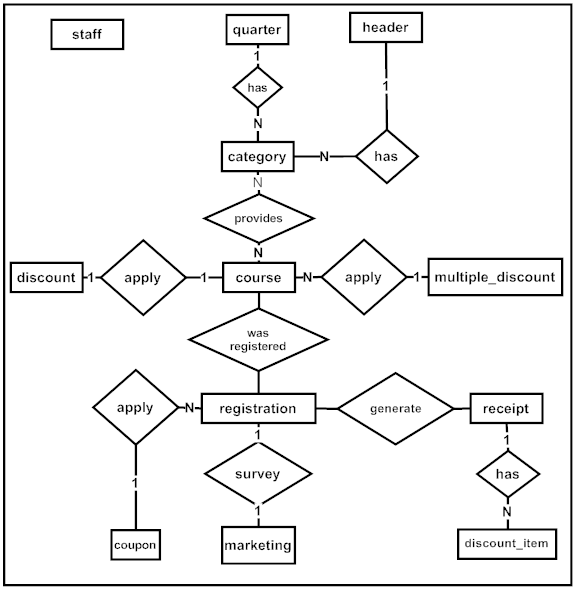
\includegraphics[height=5.3in]{images/ER_diagram.png}
    \caption{Entity Relational Diagram}
    \label{fig:er_diagram}
\end{center}
\end{figure}

\section{Database Specification}

The Key field indicates whether the column is indexed. A value of PRI indicates that the column is part of the table's primary key. UNI indicates that the column is part of a UNIQUE index. The MUL  value indicates that multiple occurrences of a given value are allowed within the column.

\subsection{Database Schema Logical Model - Relational Schema}

I'm a subsection.  This appears in the TOC.